\subsection{Especificaciones}
El variador de velocidad que se utilizó pertenece a la marca \textbf{Schneider Electric} (Figura \ref{fig:variador}) que posee las siguientes características.
	\paragraph*{Altivar 312}
	\begin{itemize}
		\item 	Modelo: ATV312HU15N4
		\item   Tensión: 380-500 V
		\item 	Frecuencia: 50/60 Hz
		\item 	Potencia: 1.5kW / 2 HP
		\item 	Fases: 3
	\end{itemize}

	\begin{figure}[h!]
		\centering
		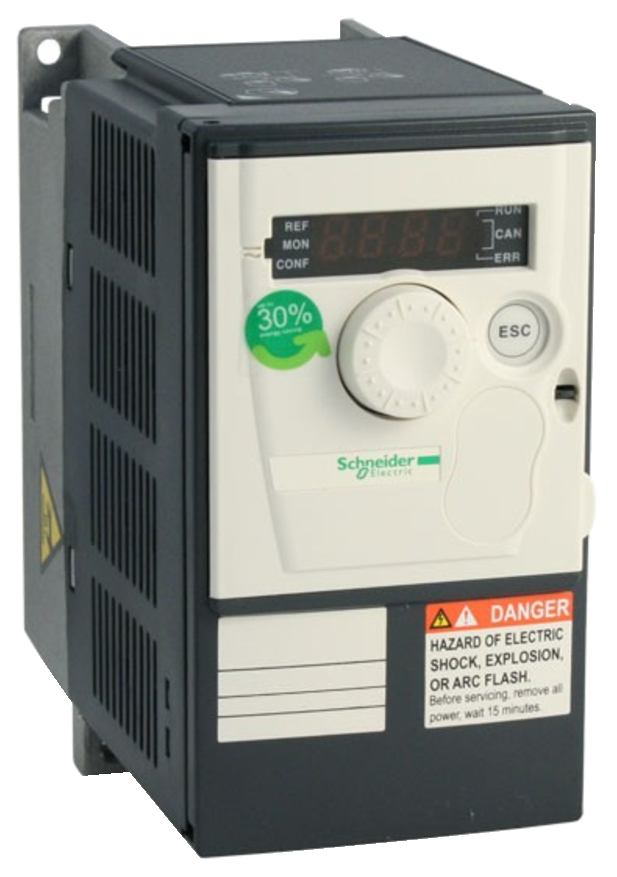
\includegraphics[scale=0.4]{variador.eps}
		\caption{Variador de velocidad Altivar 312}
		\label{fig:variador}
	\end{figure}

\subsection{Restauración de fábrica}
	Para modificar el variador desde el dispositivo se sabe que cada aceptación del parámetro o ingreso al menú se realiza presionando el botón central blanco y para buscar estos es necesario girar la misma. Para salir, tan solo presionar botón \textsl{ESC} tantas veces como sea necesarias. \\
	Para comenzar a realizar la configuración del variador de velocidad primero se procede a restaurarlo de fábrica.
	
		\begin{figure}[hbt!]
		\centering
		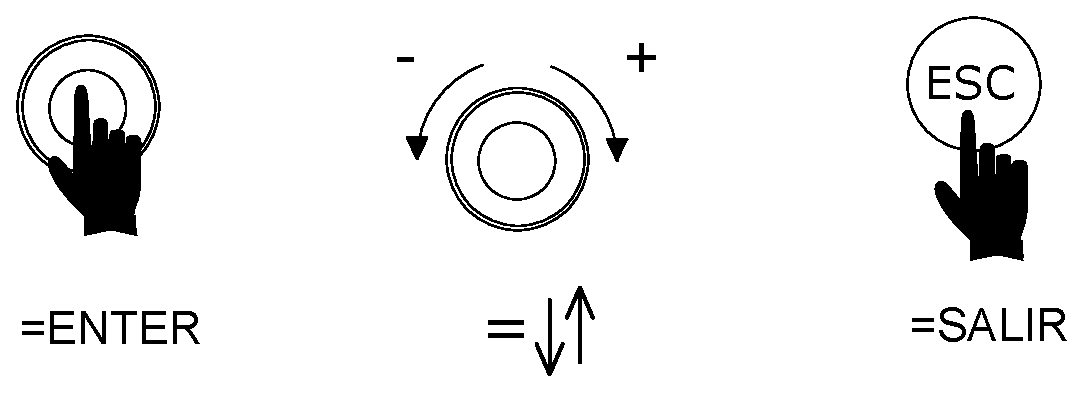
\includegraphics[scale=0.5]{ver2.eps}
		\caption{Comandos básicos del panel}
		%\label{fig:frente}
		\end{figure}
		
		\begin{figure}[hbt!]
		\centering
		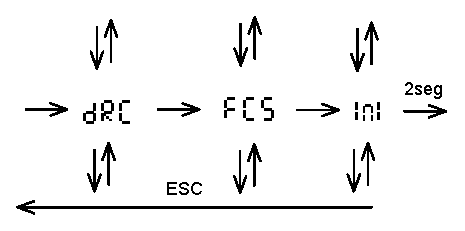
\includegraphics[scale=1]{ver1.eps}
		\caption{Restauración de fábrica}
		%\label{fig:BME280}
		\end{figure}


\subsection{Configuración de parámetros primarios}
El paso siguiente será la configuración de los parámetros del motor que se utilizará: \textsl{Frecuencia estándar del motor; tensión nominal del motor, frecuencia nominal, corriente nominal, factor de potencia}\\
\textbf{usar las imagenes en autocad}
\newpage